\chapter{When complexes overlap}
\label{ch:overlap}

This is the chapter the whole book has been deferring to, and it is the honest
one.

Every calculation in Parts~II and~III rests on one assumption, stated in
Sec.~\ref{sec:treelike} and repeated whenever it mattered: complexes meet in at
most one node. Chapter~\ref{ch:statmech} located it precisely, in the step where
a node adds what its complexes have told it as though they were independent.
The assumption is what buys the whole apparatus, and on the networks
Chapter~\ref{ch:data} measured, it is false.

So this chapter asks three questions in order. How much does the violation
cost? What would repair it? And why is the repair not simply the next chapter of
this book rather than an open problem? The answers are: less than one might
fear but not nothing; a region graph with messages on it; and because the repair
is known at the level of one network and not at the level of an ensemble, which
is the level everything else here works at.

\section{The price of treelikeness}
\label{sec:price}

Chapter~\ref{ch:chygraphs} sold the central move as follows. A triangle is a
loop, and a loop is what a tree-based calculation cannot have; promote the
triangle to a complex, sum over its interior exactly, and the loop is gone from
the outside view.

That move is real and Chapter~\ref{ch:ising} measured what it buys. But it does
not remove loops. It moves them up one level. Two triangles sharing an
\emph{edge} are a loop in the incidence structure --- a cycle through complex,
node, complex, node --- exactly as a triangle is a loop in a graph. The chygraph
cannot see it, for the same reason and by the same argument
(Fig.~\ref{fig:sharededge}).

\begin{figure}[t]
\centering
\begin{adjustbox}{max width=\linewidth}
\begin{tikzpicture}
% Two triangles sharing the edge {1,2}: a loop one level up.
\node[nd] (v0) at (-1.15,0) {};
\node[nd] (v1) at (0,0.62) {};
\node[nd] (v2) at (0,-0.62) {};
\node[nd] (v3) at (1.15,0) {};
\node[lb,anchor=east] at (-1.28,0) {$0$};
\node[lb,anchor=south] at (0,0.76) {$1$};
\node[lb,anchor=north] at (0,-0.76) {$2$};
\node[lb,anchor=west] at (1.28,0) {$3$};
\draw[lnk] (v0)--(v1) (v0)--(v2) (v1)--(v2) (v1)--(v3) (v2)--(v3);
\draw[lnk,line width=1.3pt] (v1)--(v2);
\begin{scope}[on background layer]
  \node[cx,fit=(v0)(v1)(v2)] {};
  \node[cxb,fill opacity=0.72,fit=(v1)(v2)(v3)] {};
\end{scope}
\node[lb,anchor=north,align=center] at (0,-1.35)
  {the shared edge $\{1,2\}$};
% the two countings
\node[lb,anchor=west,align=left] at (2.15,0.45)
  {\emph{Bethe}, Eq.~\eqref{eq:bethe}: $-1$ on node $1$\\
   and $-1$ on node $2$, separately.\\
   Every node counted once, but the\\
   bond $\{1,2\}$ counted \emph{twice}};
\node[lb,anchor=west,align=left] at (2.15,-0.75)
  {\emph{M\"obius}, Eq.~\eqref{eq:mobius}: $-1$ on the\\
   shared edge itself. Every node once\\
   \emph{and} every bond once};
\end{tikzpicture}
\end{adjustbox}
\caption{\textbf{A loop one level up.} Two triangles sharing an edge. Promoting
each triangle to a complex removes its internal loop from the outside view, but
the two complexes now meet in two nodes rather than one, and the cycle
complex--node--complex--node is invisible to a chygraph exactly as a triangle is
invisible to a graph. Both counting schemes count every node once; only one also
counts the shared bond once, and that is the difference between subtracting a
correlation and not.}
\label{fig:sharededge}
\end{figure}

The correct statement is therefore not that chygraphs solve clustering. It is
that they move the boundary of what counts as local, from ``no loops'' to ``no
loops \emph{between} complexes''. That is a real gain --- Chapter~\ref{ch:cover}
measured it on hyperbolic random graphs, where the degree-matched control has no
core at all and the chygraph has very nearly the right one --- and it is not the
same as a solution.

\section{Measuring the deficit}
\label{sec:deficit}

How much is left on the table can be measured, and Chapter~\ref{ch:cover}
already did most of it. On hyperbolic random graphs with maximal cliques as
complexes, the chygraph accounts for $77$ to $100$ per cent of the leaf-removal
core, with the shortfall tracking the clique overlap: negligible in a sparse
graph, where cliques rarely share edges; irrelevant once almost everything is
core; worst in between.

The sharp measurement is the \emph{rewired control} of
Sec.~\ref{sec:hrg}, and it deserves restating here because it is what licenses
the rest of this chapter. Take the measured clique ensemble and rearrange it so
that complexes meet in at most one node, holding the ensemble fixed and changing
only the arrangement. The prediction agrees with that control to $10^{-3}$. So
the map is right on its own terms, and the entire remaining discrepancy against
the real graph is overlap and nothing else. Without that control one could not
tell a wrong recursion from a violated assumption; with it, the diagnosis is
unambiguous.

\paragraph{A prior question: does the ensemble exist?} Taking maximal cliques as
complexes presumes the clique-size distribution has a limit --- specifically that
the excess cardinality $\ave{\sbar}=\ave{c^{2}}/\ave{c}-1$ of
Eq.~\eqref{eq:sbaru} converges. It is worth checking rather than assuming, and
the check separates two things.

Measured against a degree-matched control at identical degree sequence and seed,
so that $P(k)$ and assortativity are held fixed and clustering is the only
difference, the paired ratio $\ave{\sbar}_{\mathrm{HRG}}
/\ave{\sbar}_{\mathrm{control}}$ is a converged constant between $1.8$ and $4.8$
for $\tau\ge2.5$, flat over $n=10^{3}$ to $3\times10^{5}$. The clustering signal
is a multiplicative factor, not a finite-size artefact. At $\tau=2.1$ both
diverge and the control diverges \emph{faster}, so the ratio decays toward one
and nothing measured there separates clustering from the tail. That is why
Sec.~\ref{sec:hrg}'s $\tau=2.1$ row behaved differently from the others, and it
is a caution rather than a result: below $\tau=2.5$ the measured ensemble is not
converged, and neither is anything built on it.

\section{Region graphs}
\label{sec:regions}

The repair is not new physics. It is the next level of the same idea, and it has
been available since Kikuchi.

Belief propagation is exact on a tree because a tree can be decomposed into
nodes and edges with each variable counted once. When it is not a tree, the
remedy is to work with larger \emph{regions} --- sets of variables treated as
units --- and to choose counting numbers so that every variable, and every
interaction, is still counted once.

Close the complex family under intersection and assign counting numbers by
M\"obius inversion:
\begin{equation}
  c_{R}=1-\sum_{R'\supsetneq R}c_{R'}.
  \label{eq:mobius}
\end{equation}

Two things follow immediately, and the first is the reassuring one.

\emph{It contains what the book has been doing.} When complexes meet in at most
one node, the family closes on the complexes plus the single nodes, and
Eq.~\eqref{eq:mobius} gives $c_{v}=1-k$ --- precisely the counting of
Eq.~\eqref{eq:bethe}. Chapter~\ref{ch:statmech}'s free energy was a region-graph
free energy all along, on the region graph a treelike chygraph happens to have.
That is why Sec.~\ref{sec:freeenergy} could say its weights were not chosen.

\emph{It departs from it exactly where complexes overlap.} On two triangles
sharing an edge, M\"obius inversion puts $-1$ on the shared \emph{edge};
Eq.~\eqref{eq:bethe} puts $-1$ on each of its two endpoints. Both count every
node once. Only one counts the shared \emph{bond} once: summing the counting
numbers of every region containing $\{1,2\}$ gives $1$ under
Eq.~\eqref{eq:mobius} and $2$ under Eq.~\eqref{eq:bethe}. The Bethe scheme
subtracts the two shared vertices independently and so never removes the
correlation between them.

That is not a subtlety to be taken on trust. The example has four spins and can
be settled by enumeration.

\section{Two triangles, exactly}
\label{sec:twotriangles}

Couple every pair inside each triangle, evaluate $\ln Z$ exactly by summing over
all sixteen configurations, and compare.

\begin{center}\small
\begin{tabular}{rrrrr}
\hline\hline
$\beta J$ & exact & Bethe & M\"obius & GBP\\
\hline
$0.2$ & $2.8887$ & $+1.8\times10^{-2}$ & $-1.4\times10^{-3}$ & $-4\times10^{-14}$\\
$0.5$ & $3.5907$ & $+9.1\times10^{-2}$ & $-2.9\times10^{-2}$ & $-2\times10^{-13}$\\
$1.0$ & $5.7390$ & $+3.7\times10^{-1}$ & $-6.6\times10^{-2}$ & $-3\times10^{-14}$\\
$2.0$ & $10.6938$ & $+1.3$ & $-1.7\times10^{-2}$ & $-5\times10^{-15}$\\
\hline\hline
\end{tabular}
\end{center}

Three readings, in increasing order of interest.

The correction is a factor of three to eighty, so the counting matters and is
not a formality. The two schemes err in \emph{opposite} directions:
Eq.~\eqref{eq:bethe} overestimates $\ln Z$ because it never removes the
correlation between the shared vertices, and Eq.~\eqref{eq:mobius} removes it
and slightly overshoots.

And the overshoot is not a property of the counting. It is a property of
evaluating a counting on \emph{isolated} regions, which is an estimate and not a
fixed point. Running the messages removes it entirely. The last column is
generalised belief propagation in its parent-to-child form \citep{yedidia2005},
iterated to a fixed point on the region graph of Eq.~\eqref{eq:mobius}, and the
error is at the level of double precision at every coupling.

\begin{calculation}{the update that is being run}
A message lives on a directed edge of the region graph, from a region $P$ to a
direct child $R$, and is a function of the child's variables. Write
$U_{R}=\{R\}\cup\mathrm{descendants}(R)$, and $f_{R}$ for the product of every
factor whose scope lies inside $R$. The belief on a region collects every
message entering $U_{R}$ from outside it,
\[
  b_{R}(x_{R})\ \propto\ f_{R}(x_{R})
    \!\!\prod_{(I\to J):\ J\in U_{R},\ I\notin U_{R}}\!\! m_{I\to J}(x_{J}),
\]
and imposing the consistency condition $\sum_{x_{P}\setminus x_{R}}b_{P}=b_{R}$
cancels every message common to the two sides. What is left is the update:
\begin{equation}
  m_{P\to R}(x_{R})=
  \frac{\displaystyle\sum_{x_{P}\setminus x_{R}}f_{P\setminus R}(x_{P})
        \prod_{N(P,R)}m}
       {\displaystyle\prod_{D(P,R)\setminus(P,R)}m},
  \label{eq:p2c}
\end{equation}
with
\[
  \begin{aligned}
    N(P,R)&=\{(I,J):J\in U_{P}\setminus U_{R},\ I\notin U_{P}\},\\
    D(P,R)&=\{(I,J):J\in U_{R},\ I\in U_{P}\setminus U_{R}\}.
  \end{aligned}
\]
The two index sets look forbidding and are doing something simple: $N$ collects
what flows into the part of $P$ that is not $R$, and $D$ divides out what has
already been counted on the way down.

The check that this is the right generalisation is what it degenerates to. On
the two-layer region graph of a pairwise model --- one region per interaction
plus one per variable --- $D(P,R)$ holds only the edge being updated, $N(P,R)$
is the set of incoming messages to the interaction's other variables, and
Eq.~\eqref{eq:p2c} \emph{is} ordinary belief propagation. So generalised belief
propagation contains belief propagation exactly as Eq.~\eqref{eq:mobius}
contains Eq.~\eqref{eq:bethe}, and Sec.~\ref{sec:overlap-checks} reports the
numerical form of that statement.
\end{calculation}

\begin{calculation}{why it is exact here, and what that does not prove}
The region family closes on $\{0,1,2\}$, $\{1,2,3\}$ and $\{1,2\}$ once the
zero-counting singletons are dropped, and that is a junction tree: a tree of
regions in which the intersection of any two regions is contained in every
region on the path between them. Generalised belief propagation on a junction
tree is exact, for the same reason belief propagation on a tree is.

So the whole of what the table reports as left on the table is recoverable ---
but by an argument that says exactly when it is recoverable, which is when the
closed complex family is a junction tree. For maximal cliques that means the
graph is chordal, and a hyperbolic random graph is not.

One more thing this calculation settles. Generalised belief propagation refuses
to run on a region graph whose counting numbers do not cover every factor once,
and the Bethe counting on two overlapping triangles is exactly such a graph. The
failure is detected rather than silently absorbed, which is worth having: the
scheme knows the shape of its own assumption.
\end{calculation}

\section{Sixty instances, and where it stops}
\label{sec:sixty}

One example proves a possibility, not a method. Figure~\ref{fig:gbp} runs the
three schemes over sixty maximal-clique region graphs of hyperbolic random
graphs --- $n=14$, $18$ and $20$, small enough to enumerate exactly, at two
couplings, keeping only the instances that are not already treelike.

\begin{figure}[t]
\centering
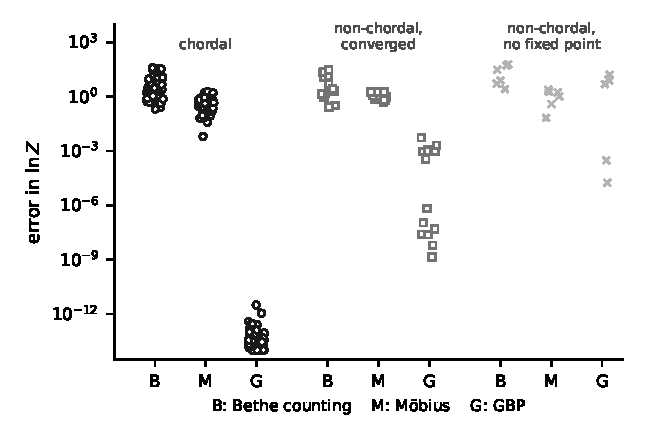
\includegraphics[width=\linewidth]{figs/fig-gbp.pdf}
\caption{\textbf{What the messages buy, and where they stop buying it.} Error in
$\ln Z$ for sixty maximal-clique region graphs of hyperbolic random graphs,
under the Bethe counting (B), the M\"obius counting evaluated on isolated
regions (M), and generalised belief propagation run to a fixed point (G).
Where the clique structure is chordal the region graph is a junction tree and
GBP is exact. Where it is not, GBP still gains two to nine orders of magnitude
--- when it converges. On six of the twenty non-chordal instances it does not
converge at all, even at damping $0.999$, and there it buys nothing. Data from
\code{probe/gbp\_cliques.py}; plotted by \code{figs/overlap.py}.}
\label{fig:gbp}
\end{figure}

The forty chordal instances come out exact, the worst error being
$3\times10^{-12}$. That is the previous section's argument holding at scale
rather than on one hand-picked example.

The twenty non-chordal instances divide, and the division is the point of this
chapter. Fourteen converge, and there the GBP error runs from
$1.4\times10^{-9}$ to $5.4\times10^{-3}$, against $0.48$ to $1.8$ for the
M\"obius counting and $0.26$ to $30$ for the Bethe counting on the same
instances --- two to nine orders of magnitude better, with the consistency
condition $\sum_{x_{P}\setminus x_{R}}b_{P}=b_{R}$ satisfied to
$2\times10^{-6}$, so what remains is the approximation's error and not the
solver's.

The other six do not converge, at any damping tried up to $0.999$. Their
residual says so, and no number from them is quoted. It is that instability,
rather than the accuracy where it converges, that matters for what comes next.

\paragraph{Two further limits, stated because the calculation is easy to
over-read.} Generalised belief propagation is not variationally bounded, so on a
region graph built from complexes that contain one another it can be
\emph{worse} than the static estimate --- covering $K_{4}$ by its four triangles
rather than by $K_{4}$ itself gives an error of $10^{-2}$ against a static
$4\times10^{-3}$. That case does not arise for maximal cliques, which never
nest, but it is a reason not to build region graphs carelessly.

And it is an \emph{instance-level} calculation. It takes an explicit list of
complexes and an explicit interaction. Everything else in this book works at the
level of an ensemble, where a message is a distribution over a chy-degree class
rather than a function on one region.

\section{Merging the offenders}
\label{sec:merging}

There is a repair more direct than a region graph, and it is worth working out
because it is the first thing anyone proposes on seeing
Fig.~\ref{fig:sharededge}: if two complexes share more than one atom, stop
treating them as two. Merge them into a single \emph{meta-complex} holding the
union of their atoms, and sum its interior exactly.

Nothing has to be added to the formalism to do this. A complex whose vertices
are complexes is what a chygraph \emph{is} --- it is the freedom
Chapter~\ref{ch:satisfiability} used to nest clauses --- and
Eq.~\eqref{eq:emitted} does not care how large or how internally tangled a
complex is, only that its interior can be enumerated. On
Fig.~\ref{fig:sharededge}'s example the merge is immediate: the two triangles
become one complex of four atoms, its $2^{4}=16$ interior states are summed
exactly, and the overlap is gone because there is nothing left for it to overlap
with. Section~\ref{sec:twotriangles}'s whole discrepancy disappears, and by a
route that needs no region graph and no parent-to-child update.

So the question is not whether the repair is correct. It is what it costs.

\paragraph{Merging is a percolation problem.} The cost is $2^{c}$ on the merged
complex, so everything turns on how large the merging grows. And that is a
question this book already has the machinery for.

Put a node on every complex, and a link between two complexes that share two or
more atoms. The meta-complexes are the connected components of that graph. The
repair is affordable exactly while that graph has \emph{no giant component} ---
and the moment it has one, the merging swallows a finite fraction of the network
into a single complex whose interior cannot be enumerated at any price.

Two details make the closure slightly more than one pass of connected
components. Merging is iterated: two meta-complexes assembled from disjoint
components can still share two atoms between their \emph{unions}, so the
procedure must be run to a fixed point. And the merged complex inherits every
inclusion of its parts, so its chy-degree is the sum --- which is what makes the
component grow.

\paragraph{What it costs on the ensemble this book is about.} Measured on
hyperbolic random graphs with maximal cliques as complexes, the answer is
discouraging and precise (Fig.~\ref{fig:merge}).

\begin{center}\small
\begin{tabular}{rrrrr}
\hline\hline
$\ave{k}$ & $n=1000$ & $n=2000$ & $n=4000$ & largest meta-complex\\
\hline
$0.3$ & $4.7$ & $5.3$ & $5.3$ & bounded\\
$0.5$ & $6.0$ & $12.3$ & $14.7$ & grows\\
$0.8$ & $19.0$ & $54.0$ & $67.0$ & grows\\
$1.5$ & $40.3$ & $208.7$ & $175.7$ & grows\\
$3.0$ & $289.7$ & $655.3$ & $1102.3$ & grows\\
\hline\hline
\end{tabular}
\end{center}

Below $\ave{k}\simeq0.4$ the largest meta-complex is a handful of atoms and does
not move with $n$: the merging terminates, the repair is exact, and it is
cheap. Above it the largest meta-complex grows with the network, reaching
twenty-eight per cent of all vertices at $\ave{k}=3$ and sixty-six per cent at
$\ave{k}=6$. At that point $2^{c}$ has an extensive exponent, which is the
original problem returned in a different costume.

\begin{figure}[t]
\centering
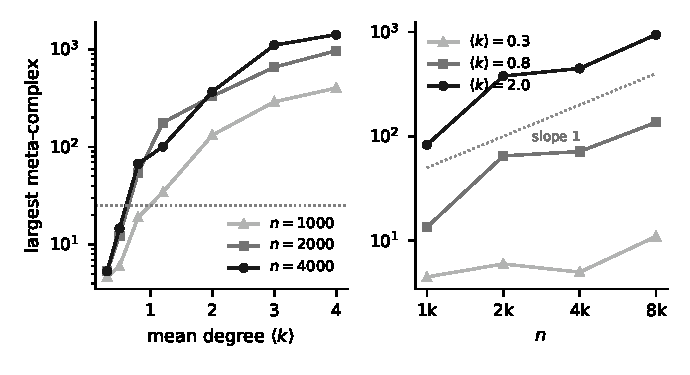
\includegraphics[width=\linewidth]{figs/fig-merge.pdf}
\caption{\textbf{When merging is affordable.} Largest meta-complex after
merging every pair of maximal cliques that share two or more atoms, iterated to
a fixed point, on hyperbolic random graphs at $\tau=2.5$. Left: against mean
degree, at three sizes; the dotted line is $2^{25}$ states, a fair limit for
exact enumeration. Right: against $n$, with a slope-one guide. At
$\ave{k}=0.3$ the largest meta-complex does not grow and the repair is exact
and cheap; by $\ave{k}=2$ it is a fixed fraction of the network. Generated by
\code{figs/merge.py}.}
\label{fig:merge}
\end{figure}

\paragraph{What to take from this.} Three things, and the first is not a
disappointment.

The repair is \emph{right}, and it is right for the reason the whole book is
organised around: a complex is allowed to contain complexes, so absorbing an
overlap into a bigger interior is a legal move rather than a patch. Where it
terminates, it gives the exact answer with no approximation anywhere and no
region graph to build.

The threshold that decides it is a percolation threshold on the overlap graph,
which is the sort of object Chapter~\ref{ch:percolation} computes. So the
feasibility of the Part~IV repair is a Part~II calculation --- one can ask, of a
given ensemble, whether merging will terminate, before attempting it. That is a
better position than discovering it by running out of memory.

And on the ensembles that motivated the construction it terminates only in the
very sparse régime. This is not special to hyperbolic graphs: clustering is
exactly what makes cliques share edges, so any ensemble with enough clustering
to need the repair tends to have enough to make it percolate. The two conditions
pull against each other, which is why Sec.~\ref{sec:whatwouldclose}'s route ---
messages between regions, rather than one enormous region --- remains the one
that scales. Merging and generalised belief propagation are the two ends of one
dial: merge everything and the messages become trivial but the interior
impossible; merge nothing and the interior is easy but the messages
approximate. Where to sit on that dial is an ensemble-by-ensemble question, and
Fig.~\ref{fig:merge} is how one answers it.

\paragraph{A practical note.} Between those extremes lies a range where merging
is worth doing on the instances one actually has, rather than on an ensemble.
Finding which complexes to merge is a mechanical, checkable operation: build the
overlap graph, take components, verify no two survivors share two atoms, verify
each is small enough to enumerate. It is exactly the kind of bookkeeping that is
tedious by hand, easy to get subtly wrong, and well suited to being automated.
A tool that took a network, proposed a merge closure, and reported the largest
interior it produced would tell a user in one pass whether the exact route is
open to them --- and the answer would be a number rather than a judgement.

\section{Clustering is a hierarchy of obstructions}
\label{sec:hierarchy}

Step back and the shape of the difficulty is visible.

A graph cannot see a triangle. Promote triangles to complexes and the chygraph
cannot see two triangles sharing an edge. Promote \emph{those} pairs to regions
and the region graph cannot see whatever loops the regions form among
themselves. Each level removes the obstruction below it and exposes the one
above. This is not a defect of the construction; it is what the cluster
variation method has always been, and the chygraph is one rung of it made
systematic and given an ensemble.

The question that decides whether the hierarchy is a solution or a regress is
whether it \emph{terminates} for the ensemble one cares about --- whether, for
maximal cliques of a hyperbolic random graph, some finite level captures
essentially all of the correlation. Section~\ref{sec:sixty} gives the shape of an
answer: the instance calculation is exact exactly when the clique structure is
chordal, so the question becomes the distribution of chordality-violating motifs
in the ensemble, and how fast their contribution decays. That is a
well-posed question about a random geometric object. It is not answered here.

\section{What would close it}
\label{sec:whatwouldclose}

The missing step can be stated precisely, which is the most this chapter can do
for it.

Every other calculation in this book carries a message per chy-degree
\emph{class}: a distribution over the ensemble, not a function on one object.
Closing the overlap deficit means lifting the parent-to-child update to a
message indexed by region \emph{type}, over a region graph that is itself a
random object. Two things would have to be supplied. What is the distribution of
intersection patterns among the maximal cliques of the ensemble --- how often do
two cliques share an edge, three cliques a vertex, and so on? And what does the
parent-to-child update become when averaged over that distribution? The
message-passing treatments that keep short loops explicitly
\citep{cantwell2019} are the natural point of comparison.

There is also a warning that the instance calculation has already delivered, and
it should be taken seriously rather than deferred. Six of twenty non-chordal
instances do not converge at damping $0.999$. An ensemble treatment inherits
that instability --- averaging does not make a divergent iteration converge ---
so damping will not be enough. It needs a schedule, or a different
parameterisation of the message, and finding one is part of the problem rather
than an implementation detail.

Until that is done, the position is the one this chapter opened with, and it is
worth stating without softening. The chygraph is exact when complexes meet in at
most one node. On the networks that motivated it they do not, and it recovers
most but not all of the answer. The size of the shortfall is measured, its cause
is identified by a control that holds the ensemble fixed, and the repair is
known on one network at a time. The ensemble version is open.

\section{Checks}
\label{sec:overlap-checks}

\emph{Against enumeration.} The two-triangle table compares three schemes with
an exact sum over sixteen configurations. The counting numbers are checked for
what they are supposed to guarantee: every node covered once by both schemes,
every \emph{factor} covered once by M\"obius and twice by Bethe on the shared
bond.

\emph{Against belief propagation.} On the two-layer region graph of a pairwise
model --- one region per interaction plus one per variable --- the
parent-to-child update reduces to ordinary belief propagation, and the
implementation reproduces an independently written one to $10^{-10}$ on a chain,
a star, a four-cycle and a theta graph. The loopy error is included, so the two
agree on the mistake as well as on the answer. That is the check that generalised
belief propagation contains belief propagation exactly as
Eq.~\eqref{eq:mobius} contains Eq.~\eqref{eq:bethe}.

\emph{Against its own fixed point.} Where the iteration converges, the
consistency condition $\sum_{x_{P}\setminus x_{R}}b_{P}=b_{R}$ holds to
$2\times10^{-6}$; where it does not, the residual reports it and the run is
discarded rather than quoted. The convergence criterion is stated rather than
implied: the residuals over the non-chordal instances fall into two clusters
separated by four orders of magnitude, and the threshold sits in the gap.

\emph{What is not checked, because it does not exist.} The ensemble version of
Sec.~\ref{sec:whatwouldclose}. Chapter~\ref{ch:outlook} lists it with the other
things this book does not do.
